\section{Framework Validation and a Bounded Decision Case}
\label{sec:framework-validation}

\subsection{RQ6: Does the Support Relation Prevent False Promotion?}

We exercised the validator with 14 in-memory claim mutations and evidence ablations. All 14 produced the expected status transition. A complete Elliptic visibility claim remained supported. Removing a required cell, a seed, or a prediction-manifest reference yielded incomplete-scope, incomplete-seed, and missing-prediction blocks. Widening Small GINE to Medium or IBM Small/Medium to Large produced a resource block rather than a performance conclusion. Integrity-failed imports, a non-independent construction alias, and construct-invalid metadata were excluded. Universal graph-harm and universal GraphSafe-improvement claims were marked refuted because observed cells contradict their quantifiers.

Figure~\ref{fig:claim-validation} compares expected and observed outcomes across the complete controlled suite.

\begin{figure}[t]
  \centering
  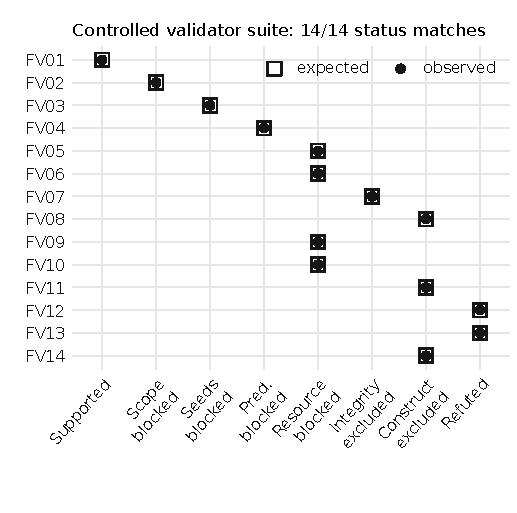
\includegraphics[width=\columnwidth]{figures/fig08_claim_support_validation.pdf}
  \caption{Expected and observed outcomes for all 14 controlled mutations. The suite checks declared support conditions; it does not prove scientific truth or ontology completeness.}
  \label{fig:claim-validation}
\end{figure}

The most consequential construct failure came from the temporal-stress package. Its runner iterates over three names, but never passes the stress argument to the benchmark harness. For each of 120 dataset--protocol--model--seed base cells, all seven performance metrics are exactly identical under the three labels. The nominal 360 rows therefore contain 120 scientific cells and 240 metadata-labeled duplicates, not three temporal conditions. We exclude the labels from stress conclusions and retain at most one deduplicated representative per base cell as supplementary rerun evidence.

A filename/count-only audit would also promote 38 integrity-failed or noncomparable result files, 20 memory-reduced GAT diagnostics, and 12 hardware-alias rows incorrectly. Across the audited families, 310 result files and 310 prediction files are at risk of such misclassification. Deterministic regeneration provides a separate check: rerunning the analysis left all 28 generated-analysis CSV hashes and all eight audited canonical input hashes unchanged. These tests establish validator behavior and reproducible derivation, not external validity or causal correctness.

\subsection{GraphSafe as a Worked Decision-Level Example}

GraphSafe combines saved graph and feature-model scores using quantities fit on training/validation data only. Its reliability risk aggregates score disagreement, rank disagreement, and entropy. A validation-selected cutoff chooses the graph score in low-risk cases and the feature score otherwise; temperatures, score thresholds, and the conservative policy gate are also set without test labels. The conservative policy can retain the validation-best branch when its reliability rules veto an override. Simple averaging and the validation-best branch are the principal comparators. The analysis uses saved predictions and performs no retraining.

\begin{table}[t]
\caption{Bounded saved-score comparison over ten seed blocks. Lower illustrative cost risk is better; no GraphSafe contrast survives Holm correction over the declared 48-test family.}
\label{tab:graphsafe}
\centering
\footnotesize
\setlength{\tabcolsep}{3.0pt}
\begin{tabular}{@{}llrrr@{}}
\toprule
Data & Method & F1 & R@1\% & Risk \\
\midrule
DGraphFin & Best val & 0.036 & 0.014 & 0.473 \\
DGraphFin & GraphSafe & 0.043 & 0.021 & 0.291 \\
DGraphFin & Average & 0.036 & 0.014 & 0.452 \\
Elliptic & Best val & 0.532 & 0.120 & 0.180 \\
Elliptic & GraphSafe & 0.533 & 0.118 & 0.178 \\
Elliptic & Average & 0.551 & 0.128 & 0.171 \\
\bottomrule
\end{tabular}
\end{table}


On DGraphFin, conservative GraphSafe has favorable descriptive means relative to simple averaging: F1 $0.0426$ versus $0.0365$, Recall@1\% $0.0209$ versus $0.0143$, and risk $0.2913$ versus $0.4522$. After averaging the six protocol--model contexts within each seed, the paired improvements are $0.00610$ F1 (95\% CI $[0.00370,0.00868]$), $0.00662$ Recall@1\% (95\% CI $[0.00402,0.00944]$), and $0.16092$ lower risk (95\% CI $[0.06409,0.28513]$). Their Holm-adjusted $p$-values in the declared 48-comparison family are 0.109, 0.0938, and 0.225.

Elliptic provides the necessary negative comparison. Simple averaging has higher mean F1 ($0.5513$ versus $0.5333$), higher Recall@1\% ($0.1276$ versus $0.1176$), and lower risk ($0.1709$ versus $0.1783$). The seed-blocked differences favor simple averaging, with adjusted $p$ between 0.0938 and 0.109 for these outcomes. No one of the 48 GraphSafe-versus-average tests has Holm-adjusted $p<0.05$.

GraphSafe is therefore useful here as a worked example of claim discipline. Its DGraphFin aggregate is promising under a declared cost and review budget; its Elliptic aggregate is worse than a cheap ensemble; and the corrected family does not support universal dominance. Temperature or prior correction should not be described as a rank repair, and the policy has not been validated as an automated AML decision rule.
